% !TEX program = xelatex
\documentclass[aspectratio=169]{beamer}
\usepackage{amsthm,amsmath,amssymb,braket,fontspec,unicode-math,multimedia}
\usepackage[absolute,overlay]{textpos}
\usetheme[numbering=none]{focus}
\usepackage[sfdefault]{CooperHewitt}

\makeatletter
\def\mdseries@sf{m} % el l m sb b eb
\def\bfseries@sf{b} % el l m sb b eb
\makeatother

% remove number from footcite
\makeatletter
\def\@makefnmark{}
\makeatletter

\setbeamerfont{title}{series=\mdseries,size=\huge}
\setbeamerfont{subtitle}{size=\Large,series=\mdseries,parent=structure}
\setbeamerfont{author}{size=\Large,series=\bfseries,parent=structure}
\setbeamerfont{institute}{size=\Large,series=\mdseries,parent=structure}
\setbeamerfont{date}{size=\Large,series=\mdseries,parent=structure}
\setbeamerfont{alerted text}{series=\bfseries}

\usepackage[backend=bibtex,url=false,doi=false,maxcitenames=1,style=authoryear]{biblatex}
\bibliography{bib}
\AtBeginBibliography{\scriptsize}

\setbeamertemplate{bibliography item}[triangle]
\graphicspath{{./figures/}}

\title{EXACTLY SOLVABLE MODEL OF CORRELATED METAL-INSULATOR TRANSITION}
\subtitle{Insights on Non-Fermi Liquid and Mott Insulator}

\author{Abhirup Mukherjee}
\institute{EPQM Seminar}

\titlegraphic{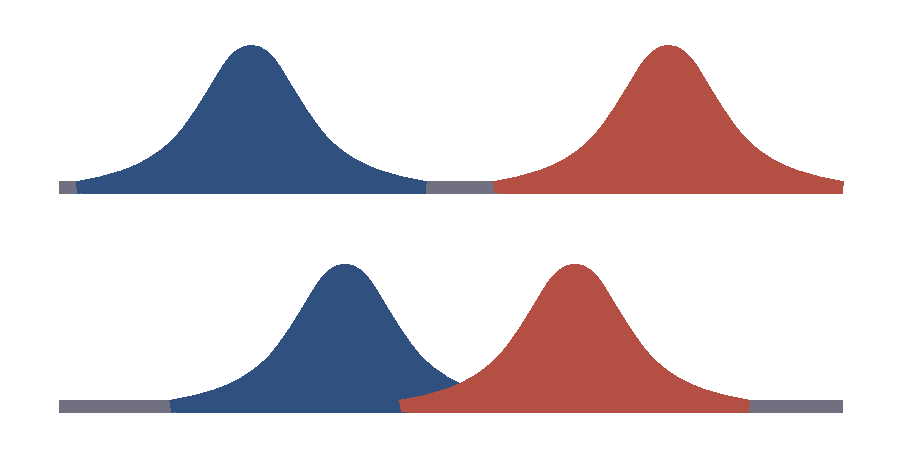
\includegraphics[width=0.4\textwidth,height=.4\textheight]{cover.pdf}}

\date{\today}
\begin{document}

\centering

\begin{frame}
\maketitle
\end{frame}

\begin{frame}{Why Are Non-Fermi Liquids Interesting ?}
	\begin{itemize}
		\item New Phase Of Matter. Beyond Landaus' theory
		\item Found in several materials, proximate to \alert{quantum critical} points.
		\item The normal state of \alert{unconventional superconductors}.
	\end{itemize}

\begin{minipage}{0.32\textwidth}
	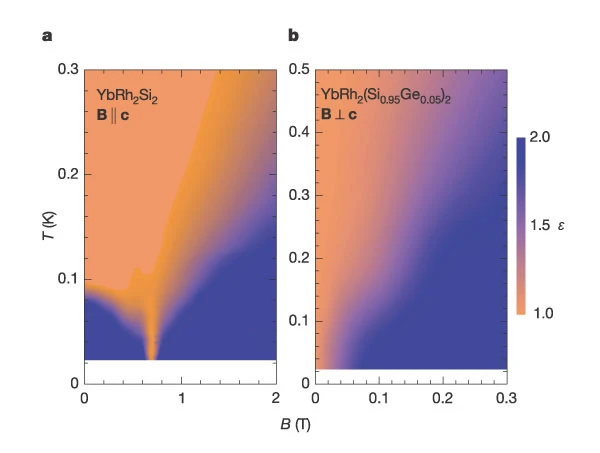
\includegraphics[width=0.9\textwidth]{heavyStrangeMetal.png}

Ge-doped YbRh$_2$Si$_2$
\end{minipage}
\begin{minipage}{0.32\textwidth}
	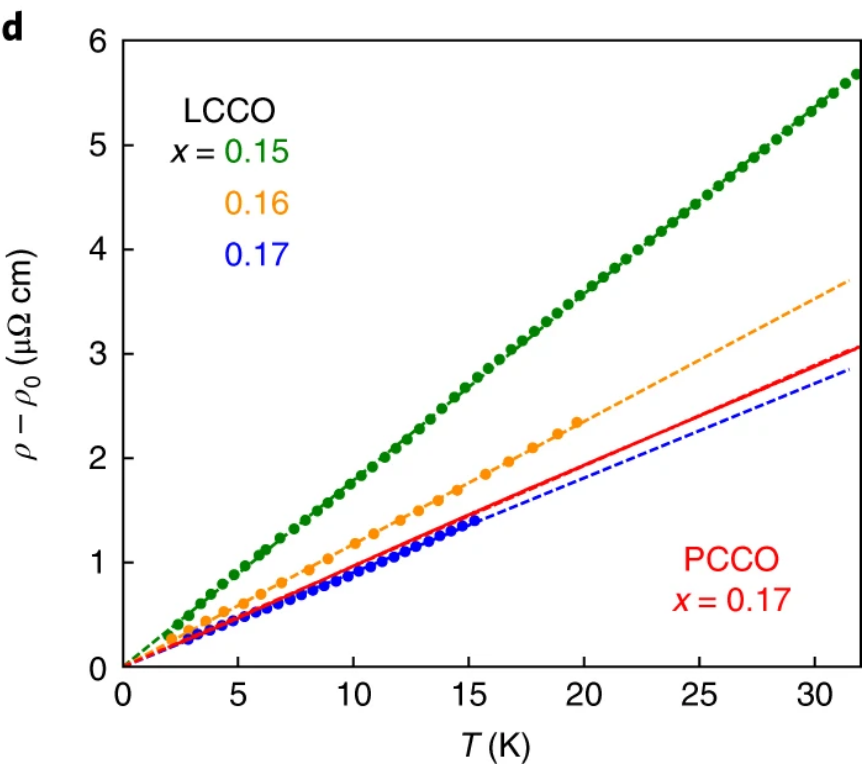
\includegraphics[width=0.9\textwidth]{cupratesStrange.png}

La$_{2−x}$Ce$_x$CuO$_4$
\end{minipage}
\begin{minipage}{0.32\textwidth}
	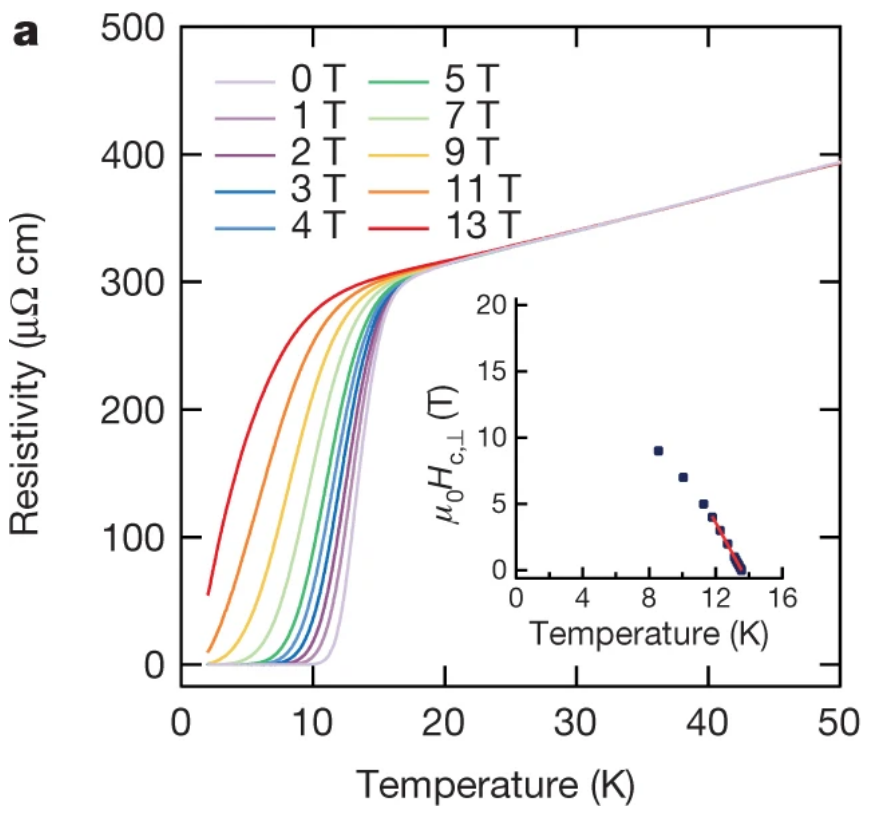
\includegraphics[width=0.9\textwidth]{nickelateStrange.png}

NdNiO$_3$, Nd$_{0.8}$Sr$_{0.2}$NiO$_3$
\end{minipage}

\footcite{Custers2003,Legros2019,SarkarStrangeMetal2020}
\end{frame}

\begin{frame}{The Hatsugai-Kohmoto Model}
	\vspace*{-10pt}
	\footcite{HatsugaiKohmoto1992,Baskaran1991}

\onslide<1->{
	Consider \alert{infinite-ranged} interaction in real-space.
	\begin{minipage}{0.6\textwidth}
	\[H = -t\sum_{\langle i,j \rangle, \sigma}c^\dagger_{i,\sigma}c_{j,\sigma} + \frac{U}{L^d}\sum_{i_1, i_2, r}c^\dagger_{i_1 + r, \uparrow}c^\dagger_{i_2 - r, \downarrow}c_{i_2, \downarrow}c_{i_1, \uparrow}\]
	\end{minipage}
	\begin{minipage}{0.35\textwidth}
	
\includegraphics[width=\textwidth]{HKM.pdf}
	\end{minipage}
}
\onslide<2->{
	Fourier transform to k-space. \alert{Decouples} into 2x2 Hamiltonians!
	\[H = \sum_{\vec k} H_{\vec k}; \quad H_{\vec k} = \varepsilon_{\vec k}\sum_\sigma n_{\vec k,\sigma} + U n_{\vec k \uparrow} n_{\vec k \downarrow}\]
}
\onslide<3->{
	Contrast with the completely \alert{local} Hubbard interaction.
	\begin{minipage}{0.6\textwidth}
	\begin{gather*}
		H_\text{int} &\sim \sum_{i}n_{i,\uparrow}n_{i,\downarrow} \\
					 &= \sum_{k_1, k_2, q}c^\dagger_{k_1 + q, \uparrow}c^\dagger_{k_2 - q, \downarrow}c_{k_2, \downarrow}c_{k_1,\uparrow}
	\end{gather*}
	\end{minipage}
	\begin{minipage}{0.35\textwidth}
		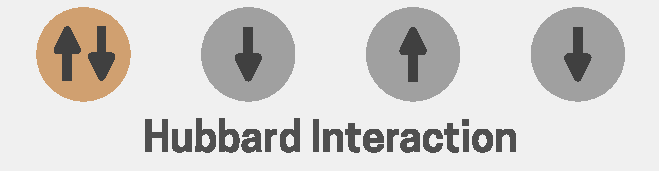
\includegraphics[width=\textwidth]{hubbard.pdf}
	\end{minipage}
}
\end{frame}

\begin{frame}{}

\vspace*{\fill}
\LARGE{\underline{THANK YOU}}

\vspace*{\fill}
\printbibliography[heading=none]
\end{frame}

\end{document}
